\documentclass[11pt,a4paper]{report}
%\usepackage[utf8]{inputenc}
\usepackage{graphicx,amsmath}
\usepackage{amsfonts}
\usepackage{amssymb}
\setlength{\tabcolsep}{20pt}
\renewcommand{\arraystretch}{1.5}

\makeatletter
\renewcommand*\env@matrix[1][\arraystretch]{%
  \edef\arraystretch{#1}%
  \hskip -\arraycolsep
  \let\@ifnextchar\new@ifnextchar
  \array{*\c@MaxMatrixCols c}}
\makeatother

\usepackage{epigraph}
\usepackage{gensymb}
\usepackage{hyperref}
\usepackage{enumitem}
\setenumerate[1]{label=[\arabic*]}
\usepackage[export]{adjustbox}
\usepackage{mathptmx}
\usepackage{tocbasic}
\usepackage{physics}
\usepackage{epstopdf}
\usepackage{subcaption}
\usepackage{tabulary}
\usepackage{placeins}
\usepackage{float}
\usepackage{morefloats}

\usepackage[a4paper,bindingoffset=0.25in,%
            left=0.5in,right=0.5in,top=1in,bottom=1in,%
            ]{geometry}
\usepackage{blindtext}
\usepackage[numbers]{natbib}
\usepackage{sectsty}
\usepackage{lipsum}
\chapterfont{\centering}
\linespread{1.3}
\begin{document}

\title{Obstacle Avoidance and Control of Autonomous Cars Using Model Predictive Control}
\author{Om Prabhu}

\begin{titlepage}
\begin{center}
        \vspace*{1in}
        {\Large \textbf{Obstacle Avoidance and Control of Autonomous Cars Using \newline Model Predictive Control\\
        }}
        \vspace*{0.4in}
        {\large \textbf{Dual Degree Project (Stage 1) Report}\\}
        \vspace*{0.4in}     
        
        \textsc{Submitted By}\\
        \vspace{.2cm}
        {\large \textbf{Om Prabhu}} \\
        {Roll No : 19D170018} \\
        \vspace*{.4in}
        \textsc{Supervisors} \\
        \vspace{.2cm}
        {\large \textbf{Prof. Avinash Bhardwaj}} \\
        {Mechanical Engineering, IIT Bombay} \\ 
        \vspace*{.2cm}
        {\large \textbf{Prof. K.S. Mallikarjuna Rao}} \\ 
        {Industrial Engineering \& Operations Research, IIT Bombay} \\
        \vspace*{0.5in}

        \begin{center}
        
\includegraphics[scale = 0.5]{iitb_logo.png}
        \end{center}
        \vspace*{0.2in}
       
        \Large{ \textbf{ INDIAN INSTITUTE OF TECHNOLOGY BOMBAY}}\\
        \vspace{.3cm}
        \large {{\textbf{Department of Mechanical Engineering}}}\\
        \vspace{.3cm}
        { October 2023 }
        \vfill
    \end{center}
\end{titlepage}
    
\clearpage
\newpage
\tableofcontents
\thispagestyle{empty}
\newpage
\pagenumbering{roman}
\listoffigures
\addcontentsline{toc}{chapter}{List of Figures}
\newpage
{\LARGE \bf Notation \& Nomenclature}

\paragraph{}
{\large
\begin{tabular}{p{0.2\textwidth} p{0.7\textwidth}}
    \textit{ACC} & Adaptive Cruise Control\\
    \textit{DARPA} & Defense Advanced Research Projects Agency\\
    \textit{DOF} & Degrees Of Freedom\\
    \textit{IPOpt} & Interior Points Optimization\\
    \textit{LIDAR} & Light Detection \& Ranging\\
    \textit{LQR} & Linear Quadratic Regulator\\
    \textit{LTV} & Linear Time-Variant\\
    \textit{MPC} & Model Predictive Control\\
    \textit{NMPC} & Non-Linear Model Predictive Control\\
    \textit{PID} & Proportional-Integral-Derivative\\
    \textit{PPC} & Pure Pursuit Control\\
    \textit{SONAR} & Sound Navigation \& Ranging\\   
\end{tabular}
}
\newpage
%\mainmatter
\thispagestyle{plain}

\pagenumbering{arabic}
\chapter{Introduction}
\section{Background of the Project}
\paragraph{}
Model predictive control (MPC) is an optimal control technique in which the calculated control actions minimize a cost function for a constrained dynamic system over a finite time horizon. It has seen major applications in the process control industry, with a major application lying in advanced process control of industrial applications such as oil refineries, kilns and boiler plants. In recent years, it has also been extensively employed in power system balancing models and in power electronics.

\paragraph{}
MPC controllers predict changes in the dependant variables of a system caused by changes in the independent variables. In most target applications, the autonomous vehicle industry alike, independent variables are often either the setpoints of PID controllers (e.g., acceleration, angular velocity) or the final control element (e.g., steering wheel, throttle/brake system). It is often a computation hassle to adjust the parameters for individual PID controllers at every time step of the process. MPC eliminates this by allowing us to model the entire control system as a single optimization problem and solve it for each finite time horizon.

\paragraph{}
While most processes are not real in the larger perspective, they can be approximately linearized over a small operating range. This allows for reduced time complexity, by reducing the time horizon of the optimization algorithm, and allows for use of the superposition principle of linear algebra. This enables the effect of changes in multiple independent variables to be added together for computation of the output response, simplifying the control problem to a series of direct algebraic manipulations that are fast and robust.

\section{Motivation for the Project}
\paragraph{}
Recent trends have witnessed a paradigm shift in the automotive industry, with a significant rise in investments on research regarding autonomous state estimation, prediction and path tracking of vehicles. The current methodology for autonomous driving control involves an explicit segregation of the driving task into lateral and longitudinal control. Lateral control systems, the most common example being adaptive cruise control, focus exclusively on the forward and backward motion of the vehicle (controlled mainly by the throttle and brake system). Longitudinal control deals with the control of steering angles for sideways motion.

\paragraph{}
The currently accepted control methodology for lateral control is using PID controllers, which calculate the throttle/brake response from an error calculation (most often based on the reference velocity. There are several methods that may be employed for longitudinal control, particularly the pure pursuit control (PPC) method and the Stanley controller. PPC involves the use of the distance between the vehicle's current position from a specific look-ahead point to adjust the controller gain, while the Stanley controller employs use of the heading and cross-track errors to determine the steering output.

\paragraph{}
In this type of segregated control system, there is almost no interaction between the lateral and longitudinal controller. This can pose severe safety risks. For example, while executing a roundabout maneuver, the vehicle's lateral controller does not always reduce the vehicle velocity before the steering wheel is turned by the longitudinal control system. Additonally, the use of multiple PID controllers can often result in computational difficulties.

\paragraph{}
The use of MPC allows both the control systems to be integrated into a single optimization problem, with the lateral control system being modeled as a set of constraints on the vehicle's lateral acceleration and velocity. The MPC algorithm can also handle non-linear systems like tire force models, allowing for accurate trajectory tracking. Finally, with some additional processing, MPC can also integrate input from the vehicle's image sensors (cameras, LIDAR and SONAR sensors) to dynamically compute obstacle constraints within the environment of the optimization problem itself. These potential benefits offer compelling reasons for the exploration for MPC as a control system for path tracking of autonomous vehicles.

\section{Report Outline}
\noindent The report structure is as follows:
\vspace{2.5mm}

\noindent \textbf{Chapter 1:} This chapter includes a brief introduction to the topic and includes the motivation for the project as well as objective for the research work.
\vspace{2.5mm}

\noindent \textbf{Chapter 2:} This chapter introduces some important theory that is used to carry out transformations from controller outputs to the dynamic states of a vehicle. This is not explicitly included as part of the code supplied with the simulations discussed in Chapter 4, but is included in the relevant function blocks.
\vspace{2.5mm}

\noindent \textbf{Chapter 3:} This chapter gives a brief literature review of previous works in MPC for autonomous vehicle path tracking, including their results, performance and limitations wherever applicable.
\vspace{2.5mm}

\noindent \textbf{Chapter 4:} This chapter discusses the current work done as part of the project, including exploration of and some adjustments to implementations of existing simulations, as well as an original model for vehicle path tracking.
\vspace{2.5mm}

\noindent \textbf{Chapter 5:} This chapter outlines the future scope and possibilities for the project.
\vspace{2.5mm}

\noindent \textbf{Chapter 6:} This chapter lists all the reference materials used so far during the project.


\chapter{Theory}
\paragraph{}
This section will discuss some important theory that is relevant to the literature and models discussed in Sections 3 and 4 respectively. The first part of the section briefly covers 2-degree of freedom vehicle dynamics and some of the existing control methods for autonomous vehicle control. The concept of model predictive control is then introduced, including the basic structure of an optimization problem involving MPC, its relevance to the control task of driving an autonomous vehicle, and a general framework for an MPC control system used in autonomous vehicles.

\section{A Brief Overview of Vehicle Dynamics}
\paragraph{}
This section discusses the kinematic and dynamic modeling of an autonomous car. A good vehicle model is essential for model-based control development, since the updates to the vehicle states rely on this model. 

\subsection{The Simple Kinematic Bicycle Model}
\begin{figure}[H]\label{fig2.1}
\centering 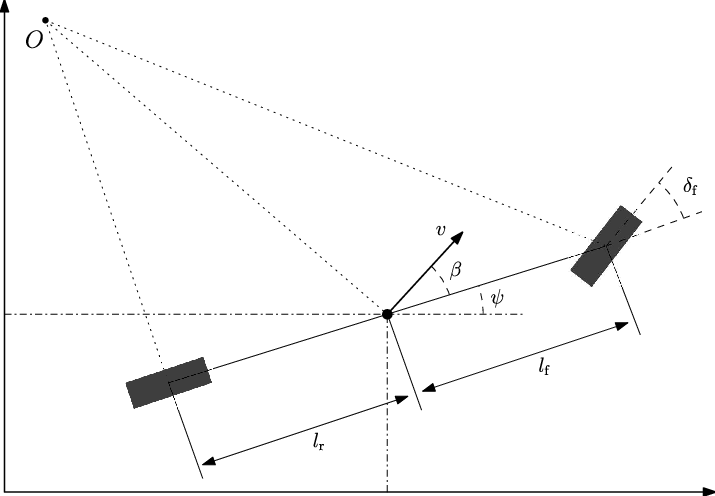
\includegraphics[scale = 0.45]{Images/simple_bicycle_model.png}
\caption{The Simple 2-DOF Bicycle Model}
\end{figure}

\paragraph{}
In most self driving control problems, the vehicle is modelled after the 2-DOF bicycle model. This is a classic kinematics model that does surprisingly well at capturing vehicle motion in normal driving conditions. This also eliminates the computational difficulties associated with other models that attempt to model the equations of each wheel separately, resulting in a highly non-linear vehicle model. Figure 2.1 illustrates the simple bicycle model with the reference point at the center of gravity. Similar models can be developed with front \& rear wheel references.

\paragraph{}
The model accepts the velocity $v$ and the rate of change of the steering angle $\varphi$ as inputs. The angle $\psi$ is known as the vehicle heading or the yaw angle. The bicycle kinematics are governed by the following set of equations:
$$\begin{array}{r}
    \text{Inputs: }\begin{bmatrix}[1] v & \varphi\\ \end{bmatrix}^T\\
    \text{States: }\begin{bmatrix}[1] x & y & \theta & \delta\\ \end{bmatrix}^T
\end{array}\longrightarrow\left\lbrace\begin{array}{l}
    \dot{x_c} = v\cos(\psi + \beta),\text{ } \dot{y_c} = v\sin(\psi + \beta)\\
    \dot{\psi} = \dfrac{v\cos\beta\tan\delta_f}{l_r+l_f},\text{ } \dot{\delta_f} = \omega\\
    \dot{\beta} = \tan^{-1}\left(\dfrac{l_r\tan\delta_f}{l_r + l_f}\right)
\end{array}\right.$$

\subsection{Modeling Vehicle States}
When dealing with vehicle states, we generally express the equations of motion in the state-space form, as follows:
$$\begin{Bmatrix}[1] \dot{x}\\ y \end{Bmatrix} = \begin{bmatrix}[1] A & B\\ C & D \end{bmatrix}\begin{Bmatrix}[1] x\\ u \end{Bmatrix}$$

\paragraph{}
The vectors $x$, $y$ and $u$ represent the states of the system, while the $A$, $B$, $C$ and $D$ matrices represent the system, input, output and feed-through respectively. The matrices for a continuous-time vehicle model are defined as follows:
$$A = \begin{bmatrix}[1]
    0 & 0 & -v\sin\psi & \cos\psi\\
    0 & 0 & v\cos\psi & \sin\psi\\
    0 & 0 & 0 & \dfrac{\tan\delta}{L_c}\\
    0 & 0 & 0 & 0
\end{bmatrix}\hspace{1cm}
B = \begin{bmatrix}[1]
    0 & 0\\
    0 & 0\\
    0 & \dfrac{v(\tan^2\delta + 1)}{L_c}\\
    0.5 & 0
\end{bmatrix}$$
where $L_c$ denotes the length of the car's wheelbase (i.e., distance from the centers of the rear wheel to the front wheel). The remaining matrices are usually defined as $C = \begin{bmatrix}[1]
    \text{I} & 0
\end{bmatrix}$, and $D = 0$. In instances of linear MPC control problems, the continuous-time model is converted into a linear model by discretizing the matrices $A$ and $B$.

\subsection{Modeling Vehicle Dynamics using Tire Parameters}
\paragraph{}
Dynamic modeling of a vehicle is more computationally complex compares to kinematic modeling, since it takes into account forces and torques acting on the vehicle. However, a dynamic model can lead to higher fidelity predictions that are not possible with kinematic models. Also, kinematic models implicitly assume a no-slip condition that is followed by the vehicle. However, at high speeds or on slippery road surfaces, this condition is not satisfied. In such cases, the throttle and steering inputs are governed by forces such as drag and friction. 

\paragraph{}
Tire modeling has been extensively researched, and there are highly non-linear models such as the Pacejka and Dugoff tire models that accurately dictate the rotational dynamics of a vehicle. In this section, however, we limit ourselves to a simpler vehicle model which uses the bicycle model discussed earlier, which is shown in Figure 2.2.

\begin{figure}[H]\label{fig2.2}
\centering 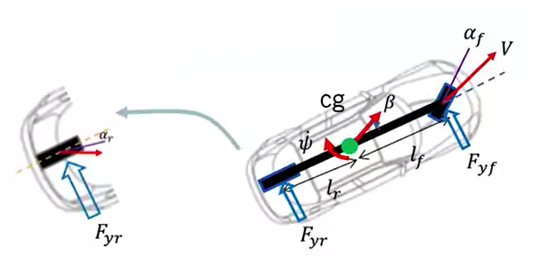
\includegraphics[scale = 1.2]{Images/vehicle_dynamics_model.png}
\caption{A Simple Vehicle Dynamics Model}
\end{figure}
\paragraph{}
The total acceleration in the inertial frame is defined as $a_y = \ddot{y}+\omega^2R=V\dot{\beta}+V\dot{\psi}$, which includes the lateral acceleration in the body frame and the centripetal acceleration. The angles $\beta$ and $\psi$ are defined as the slip angle and vehicle heading respectively. Since the only two forces affecting the lateral dynamics of the vehicle are $F_{yr}$ and $F_{yf}$, the model can now be formulated as:
\begin{align*}
    mV(\dot{\beta}+\dot{\psi})&=F_{yf}+F_{yr}\\
    I_z\ddot{\psi}&=l_fF_{yf}-l_rF_{yr}
\end{align*}
where $I_z$ denotes the vehicle's inertia about an axis perpendicular to the plane of the vehicle and passing through its center of gravity. For modeling the tire dynamics, we then introduce a linear tire model based on its front and rear tire slip angles. We define the cornering stiffness of the two wheels $C_f$ and $C_r$ as the ability of the wheels to resist deformation as the vehicle corners (i.e., the ratio of lateral force on the wheel to the tire slip angle). By modifying the above equations accordinaly, we obtain the following equations for the $A$ and $B$ matrices for the vehicle dynamics model:
$$\left.\begin{array}{r}
    \text{States: } \begin{bmatrix}[1] y & \beta & \psi & \dot{\psi}\end{bmatrix}^T\\
    \dot{X_{lateral}}=A_{lat}X_{lateral} + B_{lat}\delta 
\end{array}\right\rbrace\longrightarrow
A = \begin{bmatrix}[1]
    0 & V & V & 0\\
    0 & -\dfrac{C_r + C_f}{mV} & 0 & \dfrac{C_rl_r - C_fl_f}{mV^2} - 1\\
    0 & 0 & 0 & 1\\
    0 & \dfrac{C_rl_r - C_fl_f}{I_z} & 0 & -\dfrac{C_rl_r^2 + C_fl_f^2}{I_zV} - 1
\end{bmatrix}\hspace{5mm}
B = \begin{bmatrix}[1]
    0\\ \dfrac{C_f}{mV}\\ 0\\ \dfrac{C_fl_f}{I_z}
\end{bmatrix}$$

\section{Existing Methods for Control of Self-Driving Vehicles}
\paragraph{}
This section discusses the basic concepts regarding some existing longitudinal and lateral control techniques to control the speed of the vehicle and its steering output respectively.

\subsection{Proportional-Integral-Derivative Control}
\paragraph{}
One of the most widely used control techniques for longitudinal control of a vehicle is proportional-integral-derivative (PID) control. PID control is mathematically formulated by adding three terms dependent on the error function of the system. As the names suggest, the proportional term is directly proportional to the error $e(t)$, the integral term is proportional to the integral $\displaystyle\int_0^te(t)\text{d}t$, and the derivative term is proportional to its derivative $\dot{e}(t)$. The response of the PID controller in the time domain is expressed as follows:
$$u(t)=K_Pe(t)+K_I\int_0^te(t)\text{d}t+K_D\dot{e}(t)$$
where $K_P$, $K_I$ and $K_D$ represent the proportional, integral and derivative gains respectively. The PID control loop is illustrated in Figure 2.3.

\begin{figure}[H]\label{fig2.3}
\centering 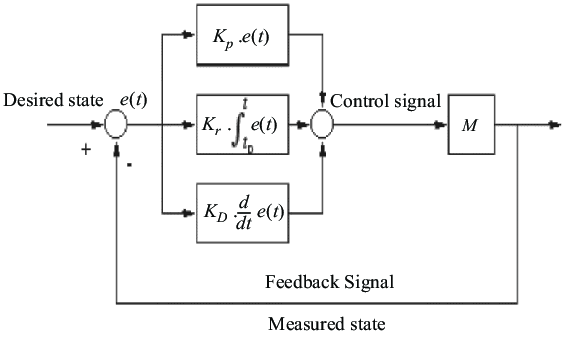
\includegraphics[scale = 0.5]{Images/pid_control_system.png}
\caption{Feedback Loop for a PID Control System}
\end{figure}

\noindent Taking the Laplace transform of the PID control equation yields the following response in the frequency domain:
\begin{align*}
    U(s) = G(s)E(s) &= \left(K_P + \dfrac{K_I}{s}+ K_Ds\right)E(s)\\
    &= \left(\dfrac{K_Ds^2 + K_Ps + K_I}{s}\right)E(s)
\end{align*}

\paragraph{}
The transfer function has only one pole at the origin, and the zeroes are located arbitrarily on the complex plane. Therefore, PID control design boils down to achieving the desired output response selecting zero locations by selecting PID gains. There are several algorithms for tuning PID gains, which will not be discussed in the report. Note that not all gains need to be used for all control systems. One or more of the controller gains can be set to zero to obtain a P, PD or PI control system.

\paragraph{}
In the context of autonomous vehicle control, PID controllers are employed for the task of cruise control. ACC systems usually employ a high level and low level controller. The high level controller is a PID controller, while the low level controller generates the throttle/brake outputs depending on the PID controller response. To maintain a desired velocity, the PID control system is set up as follows:
$$\ddot{x_{des}} = K_P(\dot{x_{ref}} - \dot{x}) + K_I\int_0^t(\dot{x_{ref}} - \dot{x})\text{d}t + K_D\dfrac{\text{d}(\dot{x_{ref}} - \dot{x})}{\text{d}t}$$

\subsection{Pure Pursuit Control}
\paragraph{}
Pure pursuit control (PPC) is a geometric path tracking control strategy used for lateral steering control. The control objective is to compute the front wheel angle $\delta$ such that the vehicle follows a given path. In the PPC method, a target point on the desired path is identified, which is a look-ahead distance $l_d$ away from the vehicle's current position. The angle $\delta$ is chosen such that the vehicle will reach the target point according to the kinematic bicycle model. Figure 2.4 illustrates the geometric aspects of PPC design.

\begin{figure}[H]\label{fig2.4}
\centering 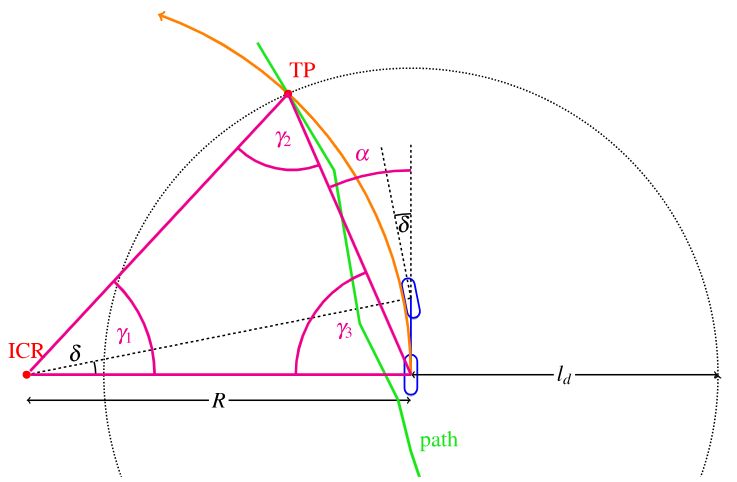
\includegraphics[scale = 0.7]{Images/ppc_diagram.png}
\caption{Geometric Aspects of Pure Pursuit Control Design}
\end{figure}
\paragraph{}
Note that the triangle formed by the instantaneous center of rotation, the target point and the vehicle's rear wheel is isosceles, which results in $\gamma_2 = \gamma_3 = 90\degree - \alpha$ and $\gamma_1 = 2\alpha$. Using the law of sines, we get the following relation between $R$ and $l_d$:
$$\frac{l_d}{\sin\gamma_1} = \frac{R}{\sin\gamma_2}\implies\frac{l_d}{\sin2\alpha} = \frac{R}{\cos\alpha}\implies l_d = 2R\sin\alpha$$

\noindent This yields the final steering output as ($L$ is the distance between the rear and front wheel centers): $$\delta=\tan^{-1}\left(\frac{2L\sin\alpha}{l_d}\right)$$

\paragraph{}
Note that the reponse of a pure pursuit controller is independent of the vehicle speed. This is ideal for ease of computations, but is likely to result in sluggish responses at high speeds and aggressive responses at very low speeds. To remedy this, the inclusion of a pure pursuit gain is proposed.
$$l_d = K_{pp}V\implies \delta=\tan^{-1}\left(\frac{2L\sin\alpha}{K_{pp}V}\right)$$

\subsection{The Stanley Controller}
\paragraph{}
The Stanley controller is another control technique used for lateral steering control of a vehicle. This controller was devised and used by the Stanford racing team in the second DARPA grand challenge. The Stanley controller makes use of the center of the front axle as the reference point, and looks at both the heading and the positional errors relative to the closest point on the path. Figure 2.5 illustrates the geometric details of the Stanley control problem.
\begin{figure}[H]\label{fig2.5}
\centering 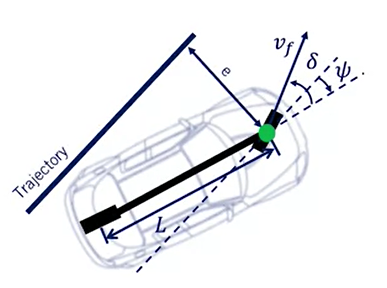
\includegraphics[scale = 1]{Images/stanley_controller.png}
\caption{Geometric Design Aspects of the Stanley Controller}
\end{figure}

\paragraph{}
The Stanley controller has three main components, which are detailed as follows:
\vspace{-2.5mm}

\begin{enumerate}[label=(\arabic*), itemsep=0em]
    \item Adjust the steering angle to align the vehicle's heading with the desired heading, i.e., $\delta(t) = \psi(t)$
    \item A proportional control is added to eliminate the cross-track error $e(t)$, whose gain is determined experimentally. The updated equation for the steering angle is: $$\delta(t) = \psi(t) + \tan^{-1}\left(\frac{ke(t)}{v_f(t)}\right)$$
    \item the steering angle must stay within the maximum and minimum bounds, i.e., $\delta\in[\delta_{min},\delta_{max}]$
\end{enumerate}

\paragraph{}
The steering angle is adjusted according to the relative magnitude of the heading and cross-track errors. The Stanley controller suffers from the same difficulty as PPC when faced with low speeds. In order to avoid an aggressive steering response, a softening constant $k_s$ is added to the control law:
$$\delta(t) = \psi(t) + \tan^{-1}\left(\frac{ke(t)}{k_s+v_f(t)}\right)$$

\section{Introduction to Model Predictive Control}
\paragraph{}
Model Predictive Control is a discrete-time multi-variable control architecture. MPC uses the current plant measurements, the current dynamic state of the process, the MPC models, and the process target variables and limits to compute the future changes in the system's dependent variables. As discussed earlier in Section 1, MPC has seen wide applications in advanced process control in chemical industries. The use of MPC is relatively new in the autonomous driving industry, and significant amount of research is being carried out to make MPC models, especially non-linear ones, implementable in real-time.

\paragraph{}
MPC is based on iterative, finite-time horizon optimization of a plant model. At time $t$, the current plant state is sampled and a cost minimizing control prediction is computed for a relatively short time horizon $[t, t+T]$. This is known as the prediction horizon. A numerical minimization algorithm is used to compute the optimal control strategies for all the time intervals starting from the current time up to the prediction horizon. 

\paragraph{}
The control horizon, on the other hand, is the section of the prediction horizon in which control moves are allowed. This is different from the prediction horizon, in that the optimal control strategy is only computed across the prediction horizon, while the control inputs are actually manipulated in the control horizon. A general rule of thumb is to set the control horizon to around 10-20\% of the prediction horizon.

\paragraph{}
Once the optimal control strategies have been computed by the optimization algorithm, the MPC controller implements only the first control strategy. The plant state is then sampled again and the calculations described above are repeated for the new current state, yielding a new set of optimal control strategies and new predicted state path. The prediction horizon keeps shifting forward as the MPC algorithm proceeds, which makes MPC an example of receding horizon control. Figure 2.6 illustrates a basic MPC control loop. 
\begin{figure}[H]\label{fig2.5}
\centering 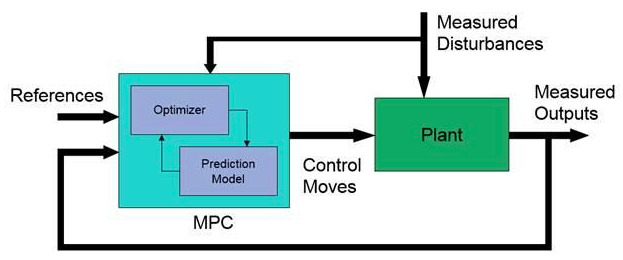
\includegraphics[scale = 0.6]{Images/mpc_control_loop.png}
\caption{Basic MPC Control Loop}
\end{figure}

\paragraph{}
Model predictive control is, hence, a multi-variable control algorithm that uses an internal dynamic model of the process, a cost function $J$ over the receding horizon, and an optimization algorithm minimizing the cost function $J$ using the control input $u$. An example of a quadratic cost function for the MPC optimization problem is given by:
$$J=\sum_{i=1}^Nw_{x_i}(r_i-x_i)^2+\sum_{i=1}^Mw_{u_i}\Delta u_i^2$$
\vspace{-12.5mm}

\begin{align*}
    \text{where }\text{ }\text{ }\text{ }x_i&: i^{\text{th}}\text{ controlled variable}\hspace{0.7\textwidth}\\
    r_i&: i^{\text{th}}\text{ reference variable}\hfill\\
    u_i&: i^{\text{th}}\text{ manipulated variable/control input}\hfill\\
    w_{x_i}&:\text{weighting coefficient reflecting the relative importance of }x_i\hfill\\
    w_{u_i}&:\text{weighting coefficient penalizing relative big changes in } u_i\hfill
\end{align*}

\paragraph{}
LQR is another optimal control method that has a quadratic cost function. While MPC looks at weighted sets of error functions, the LQR algorithm looks at all linear system inputs and computes a transfer function that minimizes the total error. Further, LQR optimizes over the entire time window and the same solution is often employed for the entire operating time, while MPC optimizes over a receding time horizon. Due to these fundamental differences, MPC is likely to obtain sub-optimal solutions for some time steps. However, since MPC makes no assumptions about linearity of system inputs, it can handle hard constraints. This difference is discussed in greater detail in section 3.2.

\subsection{General MPC Framework for Self-Driving Vehicles}
\paragraph{}
Model predictive control can be employed in several autonomous driving applications, both for lateral as well as longitudinal control, to improve vehicle responsiveness while maintaining passenger safety and comfort. Some features of MPC that are useful for autonomous driving are:
\vspace{-2.5mm}

\begin{itemize}[itemsep=0em]
    \item MPC can explicitly handle input and output constraints, which makes it very easy to impose limits on speed \& acceleration limits, safe following distance, steering angle \& steering rate limits, and constraints regarding obstacles in the vicinity of the vehicle
    \item MPC uses an internal model of vehicle dynamics to predict the behaviour of the ego vehicle across a receding time horizon. This enables the system to preview reference trajectories and disturbances over the prediction horizon.
    \item Adaptive MPC allows updating of the internal vehicle model at run time. This is especially useful in cases where the dynamics of the ego vehicle vary with time, such as for velocity-dependant steering dynamics. 
\end{itemize}

\paragraph{}
MPC also deals with several drawbacks of classical control systems. Firstly, it integrates the lateral and longitudinal control instead of treating them as separate aspects of the self-driving task. It also does not require any tuning of controller gains, which may be a difficulty in traditional control systems making use of several PID controllers along with Stanley/PPC controllers. Finally, it can handle constraints on control inputs, vehicle states and obstacles directly as part of the optimization problem instead of employing a separate system that deals with environmental input from image sensors on the car.

\paragraph{}
A common driving task where MPC is employed is path tracking and obstacle avoidance. The following optimization problem setup can be used for the above driving scenarios:
\begin{align*}
    \min_{x_{1:T}, u_{1:T}} & J(x_{1:T}, u_{1:T}) = \sum_{t=1}^T e^{\prime}Qe + u^{\prime}Ru\\
    \text{s. t. }\text{ }\text{ } & x_{t+1} = f(x_t, u_t)\hspace{31.5mm}\forall t\in[1, T-1]\\
    & \dot{x}_t\in[\dot{x}_{min}, \dot{x}_{max}]\hspace{32mm}\forall t\in[1, T]\\
    & u_t\in[u_{min}, u_{max}],\text{ }\dot{u}_t\in[\dot{u}_{min}, \dot{u}_{max}]\hspace{5mm}\forall t\in[1, T]\\
    & u_t\in\mathcal{U}_t,\text{ }x_t\in\mathcal{X}_t\hspace{30mm}\forall t\in[1, T]\\
    & \text{(obstacle \& other constraints)}
\end{align*}

\noindent where $e=\abs{x_{ref}-x}$ represents the error in reference tracking, $Q$ and $R$ represent the weighting matrices for the trajectory error and vehicle inputs respectively, and $\mathcal{X}_t$ \& $\mathcal{U}_t$ represent the range space of the vehicle states and inputs respectively. $\mathcal{X}_t$ and $\mathcal{U}_t$ together are often referred to as the vehicle's operational design domain (ODD).

\paragraph{}
Of course, this list of constraints is not exhaustive, and more constraints can be added as necessary. For example, certain driving applications might necessitate constraints on the vehicle's acceleration. The vehicle might also encounter obstacles only after a certain time has passed, in which case, the constraints have to be dynamically added to the model. The use of MPC for various driving applications is illustrated in Section 4.

\chapter{Literature Review}
\section{Lin et al (2018) \cite{lin2018adapting}}
\paragraph{}


\paragraph{}


\paragraph{}


\paragraph{}


\subsection*{Matlab data processing}


\paragraph{}


\section{Wang and Nuttall (2010) \cite{wang2010phase}}


\paragraph{}

\chapter{Current Work}
\noindent \underline{\textbf{Note:}} Some models discussed in this section have certain functions and function blocks that are derivative of existing custom Simulink$^{\circledR}$ libraries and code excerpts from GitHub repositories. In such a case, the relevant sources have been duly cited wherever appropriate.

\paragraph{}
This section discusses several optimization models for predictive control for self-driving cars. The first sub-section briefly covers re-implementations of some existing models in Simulink$^{\circledR}$ in order to explore the characteristics of an MPC controller and the effect of design parameters on model response. The second sub-section illustrates a Python implementation of an MPC controller for obstacle avoidance.

\paragraph{}
The discussions in this section are mostly limited to the results and performance of the models, and code excerpts are provided wherever necessary. A detailed code implementation of all the simulations discussed below can be found in the following GitHub repository: \href{https://github.com/omprabhu31/mpc_self_driving_cars}{\texttt{omprabhu31/mpc-self-driving-cars}}.

\section{Re-implementation of existing models}

\subsection{Basic MPC controller model for lateral and steering control}
\paragraph{}
This section discusses the implementation of a basic MPC controller that has been designed to control an autonomous vehicle steering system. The driving task consists of performing a smooth overtake maneuver without having a very high rate of change of the steering angle. Note that the only feedback to the MPC controller is the plant output (i.e., the lateral position and yaw angle). The vehicle states (i.e., velocity, heading and position coordinates) are not part of the feedback loop. As a result, it is not possible for this type of MPC controller to handle varying velocity input. The control loop for this scenario has been illustrated in Figure 4.1.

\paragraph{}
The simulation discussed above has been implemented by consulting a web-based Mathworks tutorial$^{\text{[4]}}$ available on the Internet. The `reference signal' and `plant' simulation blocks have been used directly from a Simulink$^{\circledR}$ library called \texttt{Meldas\_library}. These blocks provide functions for transformation of the controller output (i.e., the steering angle) to the plant output using standard vehicle dynamics equations.

\begin{figure}[H]\label{fig4.1}
\centering 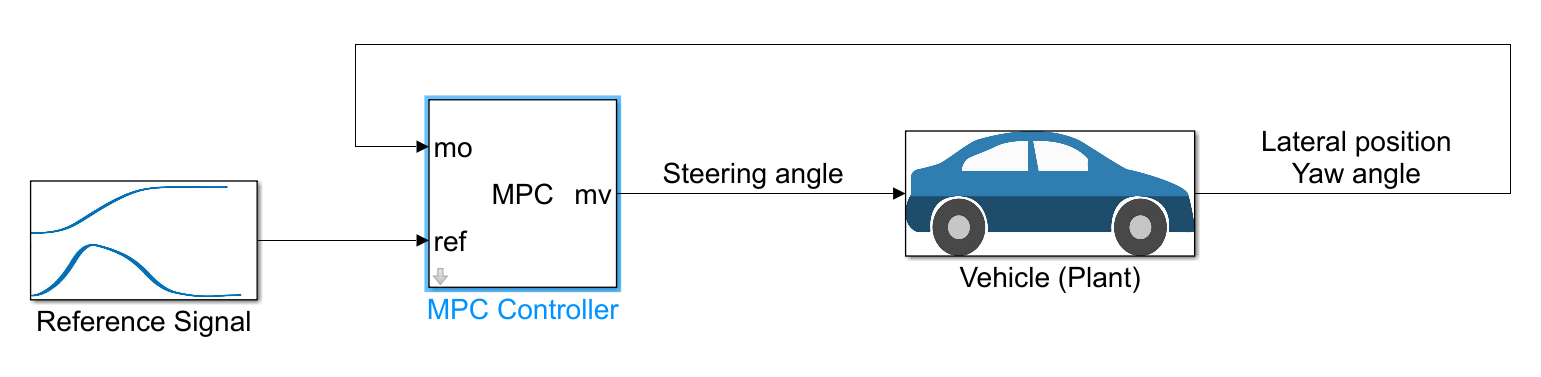
\includegraphics[scale=0.4]{Images/basic_mpc_model.png}
\caption{Basic MPC Control Loopn for Autonomous Vehicle Control}
\end{figure}

\begin{figure}[H]\label{fig4.2}
\centering 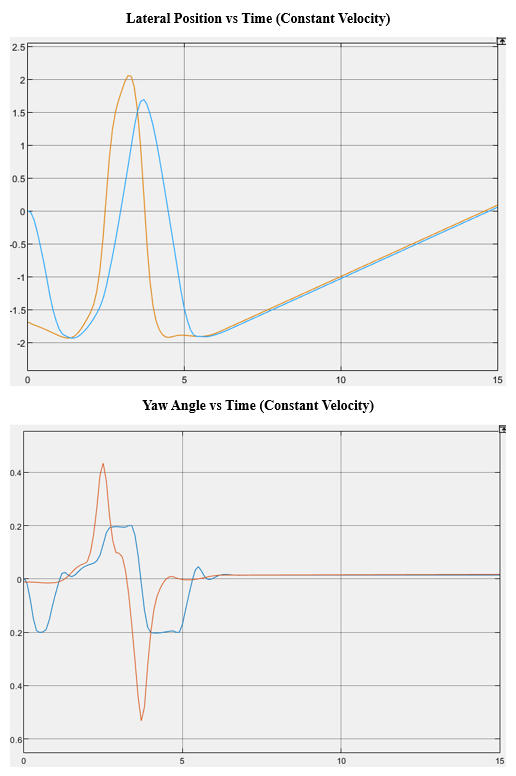
\includegraphics[scale=1.1]{Images/basic_mpc_constant_response.png}
\caption{Basic MPC Controller Response to Constant Velocity Input}
\end{figure}
\paragraph{}
Figures 4.2 and 4.3 illustrate the response of this control system to a fixed velocity input and a sinusoidal velocity input respectively. As observed, the controller has near perfect tracking for a constant velocity input. If the desired velocity or prediction horizon is increased, the controller displays a somewhat tardy response, but still provides an acceptable response for a basic overtake maneuver. 

\paragraph{}
However, for a time-varying velocity input, the controller response is not ideal. The control output (i.e., steering angle) and plant output both diverge with time. To tackle this problem involving varying velocity, we need to implement an adaptive MPC controller which allows for feedback of vehicle states back to the controller.

\begin{figure}[H]\label{fig4.3}
\centering 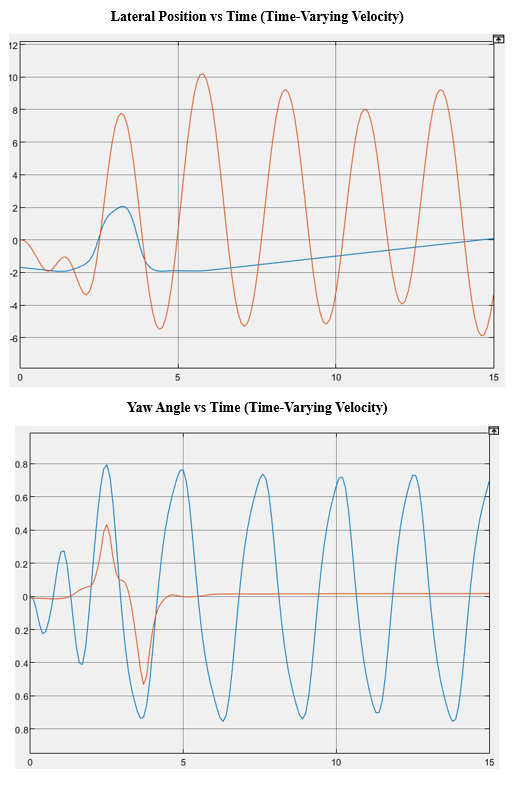
\includegraphics[scale=1.1]{Images/basic_mpc_varying_response.png}
\caption{Basic MPC Controller Response to Varying Velocity Input}
\end{figure}

\subsection{Adaptive MPC controller model for lateral and steering control}
\paragraph{}
This section discusses the implementation of an adaptive MPC controller that has been designed to control an autonomous vehicle steering system. The driving task still remains that of performing an overtake maneuver. The control loop for this scenario has been illustrated in Figure 4.4. Note that, unlike the basic MPC controller, we also introduce the vehicle states as feedback to the controller. Hence, it is possible for us to implement control of vehicle velocity as well as steering angle by updating the vehicle dynamics model at each time step.

\paragraph{}
The above simulation has been implemented by consulting a web-based Mathworks tutorial$^{\text{[5]}}$ available on the Internet. The `reference signal' and `plant' simulation blocks have been used directly from a Simulink$^{\circledR}$ library called \texttt{Meldas\_library}. These blocks provide functions for transformation of the controller output (i.e., the steering angle) to the plant output using standard vehicle dynamics equations.

\paragraph{}
The \texttt{tf\_fn} block carries out a transformation from the vehicle states to the state-space matrices of the vehicle model. It makes use of standard vehicle dynamics equations involving the vehicle parameters, states and controller sample time to compute a discrete-time plant model.

\begin{figure}[H]\label{fig4.4}
\centering 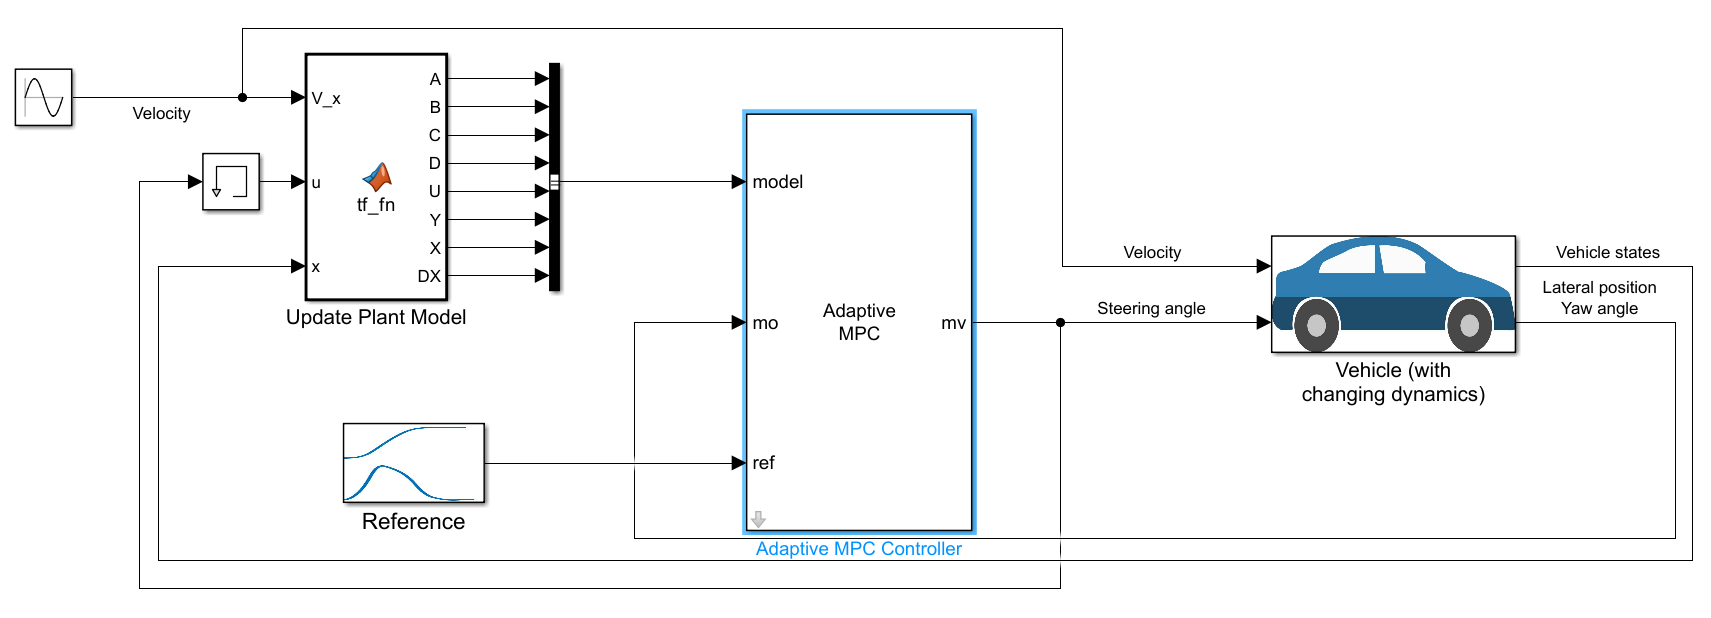
\includegraphics[width=\textwidth]{Images/adaptive_mpc_model.png}
\caption{Adaptive MPC Control Loop}
\end{figure}

\paragraph{}
As expected, the output response in case of a constant velocity is identical to that of the basic MPC controller (refer to Figure 4.2 for output response plots). Figure 4.5 illustrates the response of the adaptive MPC control system to a time-varying velocity input. For simulation purposes, we have employed a sample-based sinusoidal velocity input, but the controller performs just as well for any other varying velocity function. While the traditional MPC controller discussed in the previous section failed to track a time-varying velocity input, the adaptive MPC model is able to satisfactorily track a sinusoidal velocity input. 

\paragraph{}
This example illustrates the effectiveness of an adaptive MPC controller to take into account changing plant dynamics as part of the controller feedback loop. Note that the output response for the yaw angle does deviate slightly compared to the reference signal - this is because we have employed constrained on the maximum and minimum values of the yaw angle as well as yaw rate in order to avoid sudden jerks.

\begin{figure}[H]\label{fig4.5}
\centering 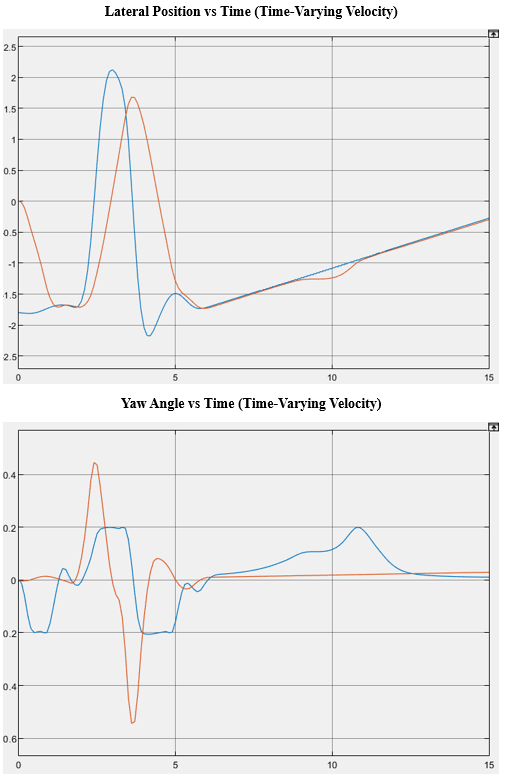
\includegraphics[scale=1.1]{Images/adaptive_mpc_varying_response.png}
\caption{Adaptive MPC Controller Response to Sinusoidal Velocity Input}
\end{figure}

\subsection{MPC controller model for path tracking across a racetrack}
\paragraph{}
This section discusses a the implementation of an adaptive MPC controller that has been designed to traverse a given racetrack. Because performing steering maneuvers along sharp turns is one of the major challenges faced in autonomous steering control, we select a track comprising two circular loops placed adjacent to each other, mimicking a figure-eight shape. The driving task is to traverse the path with reasonable accuracy.
\newpage

\paragraph{}
The simulation of a vehicle traversing a figure-eight loop involves the following steps:
\begin{enumerate}[label = (\arabic*), itemsep=-0.3em]
    \item defining the reference points for the figure-eight track by specifying the radius of the circular loops and step size of angles to be traversed
    \item calculating the reference pose and curvature vectors using the linearized distance vectors
    \item transforming the vehicle parameters and state variables (velocity, torque, etc) to compute the state-space matrices for the vehicle dynamics model
    \item compute the curvature function to maintain the vehicle along the curved path
\end{enumerate}

\paragraph{}
The control for this driving scenario is illustrated in Figure 4.6. Note that this model employs the use of 3-degree of freedom vehicle dynamics instead of the simple 2-degree of freedom bicycle model discussed earlier in Section 2. At the current stage, this lies outside the scope of the project and hence, the code for the same been adapted from an online Mathworks repository$^{\text{[6]}}$. This includes the parts of the simulation involving the powertrain \& driveline system and the transformation functions for mapping vehicle states to the 3-DOF model parameters. 

\begin{figure}[H]\label{fig4.6}
\centering 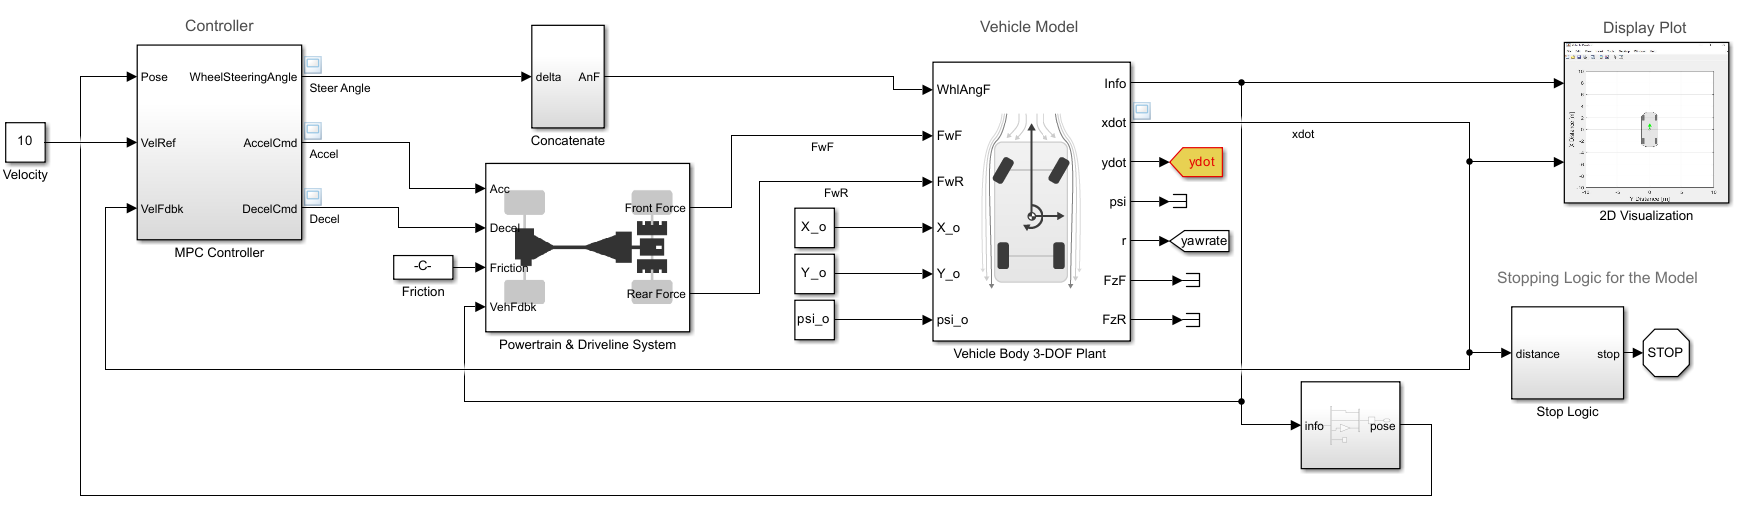
\includegraphics[width=\textwidth]{Images/figure_eight_model.png}
\caption{Control Loop for Path Tracking Along a Racetrack}
\end{figure}

\paragraph{}
Figures 4.7 and 4.8 illustrate the response of the above control system to various operating conditions (red plot represents reference trajectory, black plot represents model response). As observed, the performance of the MPC controller is near perfect for tracking the reference trajectory at reasonably low values of desired vehicle velocity. As we increase the desired velocity, the controller displays a tardy response and the trajectory tracking output is significantly worse. This is an expected behaviour, since the task of turning corners or performing roundabout maneuvers is significantly more difficult at higher speeds even with current manual control vehicles. As is seen in Figure 4.8, the model struggles to keep up with the reference trajectory at high velocities. In fact, setting the vehicle speed to 30 m/s causes the MPC algorithm to reach an infeasible solution while tracking the loop.

\paragraph{}
Note that the model discussed above only allows for a fixed vehicle speed. However, in real life, we rarely wish to perform sharp turning maneuvers at fixed speeds. To counter this problem, we can instead employ an adaptive MPC controller in order to include the vehicle states as part of the feedback control loop. This potential improvement to the model is discussed in greater detail in Section 5 of the report.

\begin{figure}[H]\label{fig4.7}
\centering 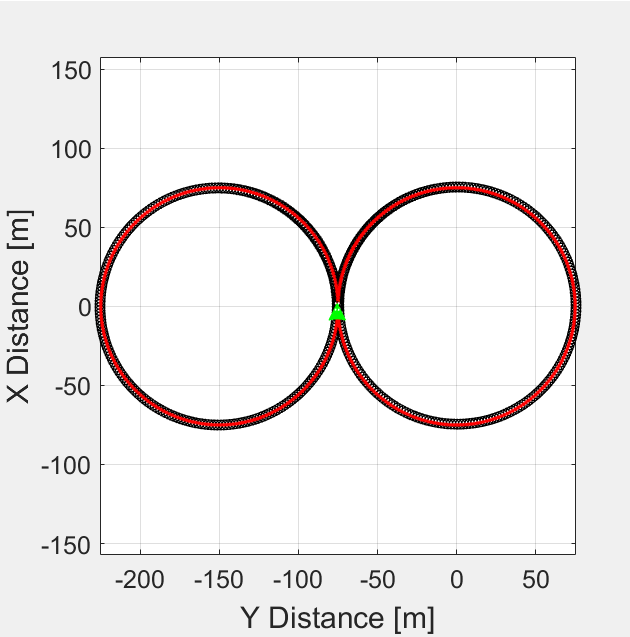
\includegraphics[scale=0.8]{Images/low_velocity_tracking_response.png}
\caption{Vehicle Path Tracking Response for Low Reference Velocity (10 m/s)}
\end{figure}

\begin{figure}[H]\label{fig4.8}
\centering 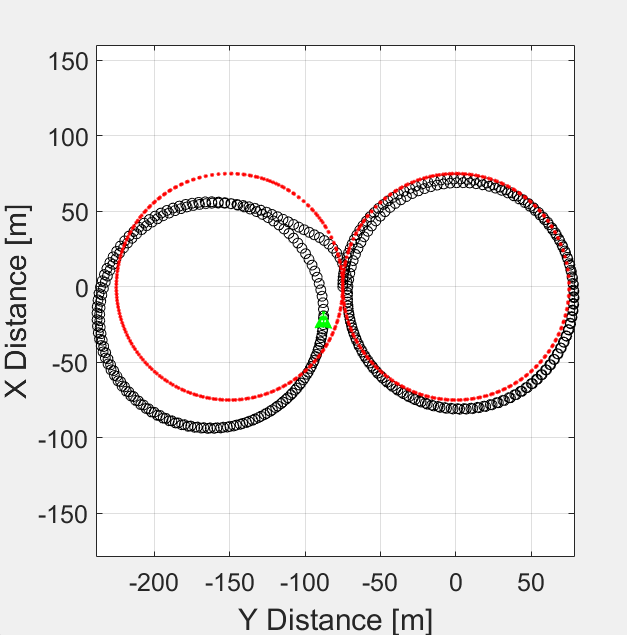
\includegraphics[scale=0.8]{Images/high_velocity_tracking_response.png}
\caption{Vehicle Path Tracking Response for High Reference Velocity (25 m/s)}
\end{figure}

\subsection{MPC controller model for generation of obstacle constraints}
\paragraph{}
This section discusses the implementation of an adaptive MPC controller for dynamic generation of obstacle constraints. The simulation initially starts out with an empty set of constraints (barring the constraints on velocity and steering angle) and updates them upon detection of an obstacle based on several parameters such as obstacle \& safe zone dimensions, detection distance and distance of the vehicle from the obstacle. The driving task is straightforward - the vehicle must avoid the obstacle (and preferably also avoid entering the safe zone) by switching to the adjacent lane and then coming back to it's original lane. Without loss of generality, we assume that the vehicle always shifts into the left lane to avoid the obstacle. The control loop for this driving scenario is illustrated in Figure 4.9.

\paragraph{}
Some aspects of the code for this simulation have been adapted from a web-based Mathwork's tutorial$^{\text{[7]}}$, including code for plotting the obstacle avoidance maneuver and relationships between some of the simulation blocks used to store vehicle states and for passing the generated constraints to the adaptive MPC controller. 

\begin{figure}[H]\label{fig4.9}
\centering 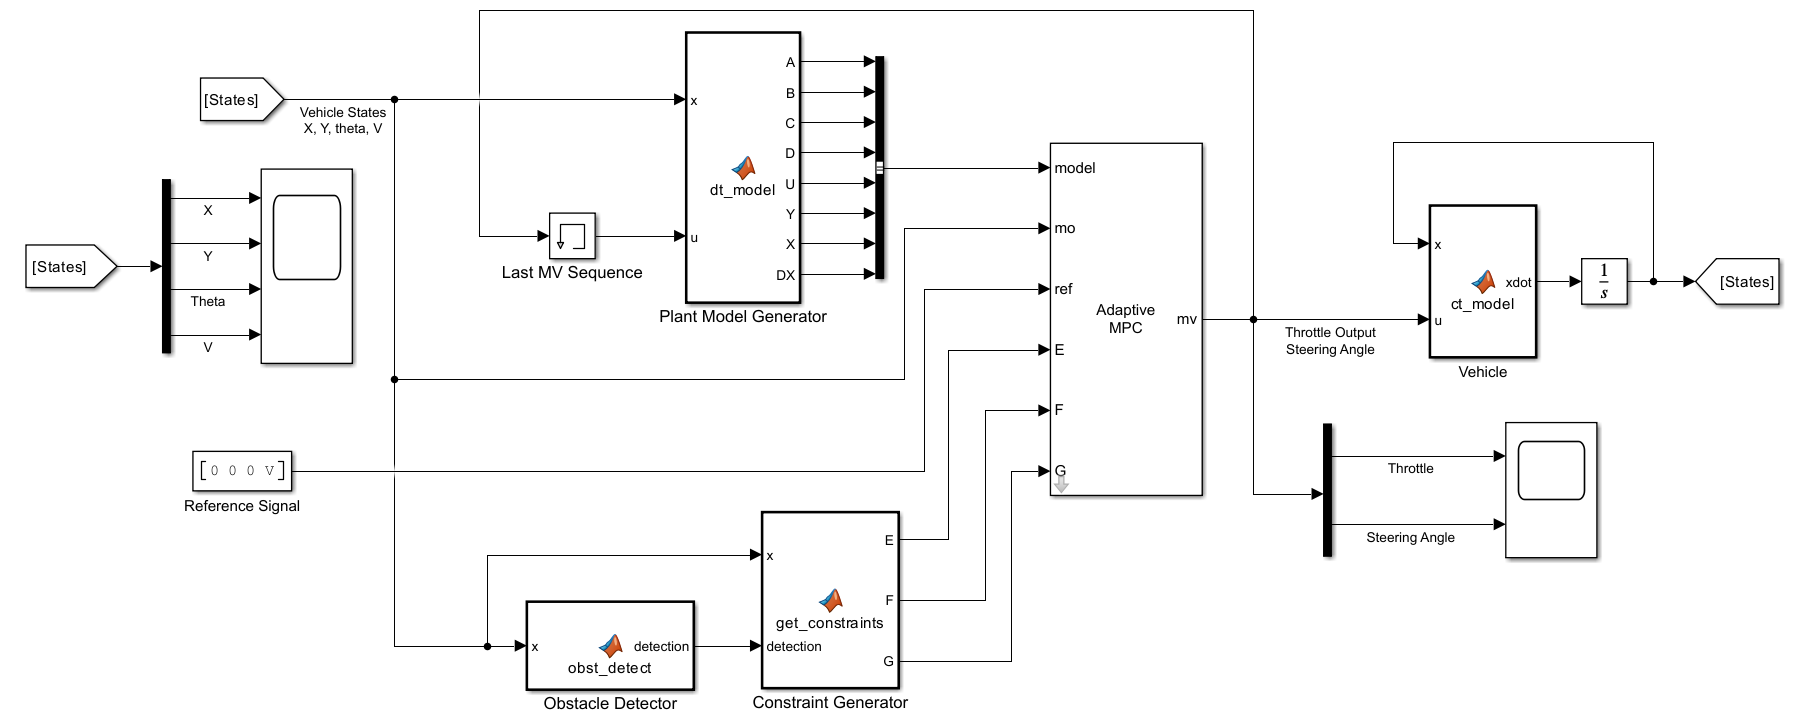
\includegraphics[width=\textwidth]{Images/obstacle_avoidance_model.png}
\caption{Adaptive MPC Control Loop for Obstacle Avoidance}
\end{figure}

\paragraph{}
Apart from the velocity and steering angle constraints, we dynamically compute the obstacle constraints at each time step. This is done as follows:
\begin{enumerate}[label = (\arabic*), itemsep=-0.3em]
    \item As the vehicle travels along its path, the distance between the vehicle and the obstacle decreases until it hits the obstacle detection distance
    \item Once the vehicle detects the obstacle, it computes a safe zone around the obstacle
    \item For every time step, we impose the following constraints:
    \begin{enumerate}[label = (\roman*), itemsep=-0.3em]
        \item vehicle must not collide with the obstacle (hard constraint)
        \item vehicle must not enter the safe zone as far as possible (soft constraint)
        \item draw a hypothetical line passing through the nearest corner of the safe zone and the current position - the vehicle must not cross the region to the right of this line (soft constraint)
    \end{enumerate}
\end{enumerate}

\paragraph{}
Depending on the vehicle's starting velocity, it may or may not end up violating the soft constraints. For example, if the starting velocity of the vehicle is very high, it will be unable to decelerate in time - this is because we have also imposed constraints on the rate of acceleration to avoid sudden jerks in the response. In such a case, the vehicle may violate the safe constraints and cross into the obstacle's safe zone and/or the partition defined by the third constraint.

\begin{figure}[H]\label{fig4.10}
\centering 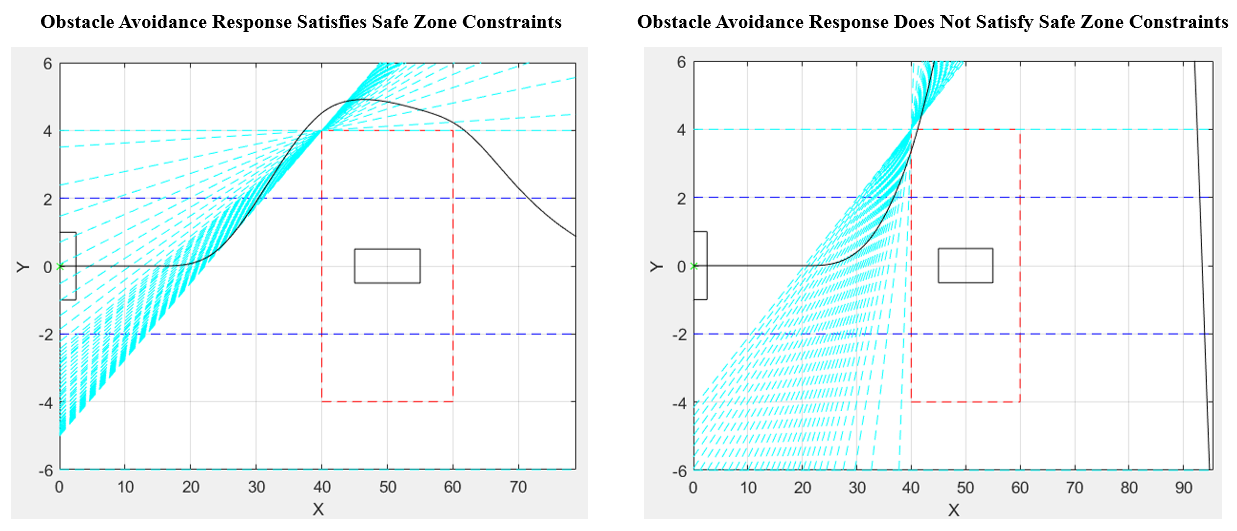
\includegraphics[width=\textwidth]{Images/satisfies_and_violate_safe_zone.png}
\caption{Variation of Obstacle Avoidance Response with Initial Velocity}
\end{figure}

\paragraph{}
The prediction horizon also has a considerable effect on the output response. In general, the longer the prediction horizon, the smoother the output response. This is because the optimization is solved for a larger number of future time steps. As illustrated in Figure 4.11, the simulation with the smaller prediction horizon displays a much tighter output response. It also crosses into the safe zone while returning back into its original lane. On the other hand, the simulation with the larger prediction horizon provides a much smoother and generally safer obstacle avoidance maneuver. However, a large prediction horizon may cause computational difficulties in some cases.

\begin{figure}[H]\label{fig4.11}
\centering 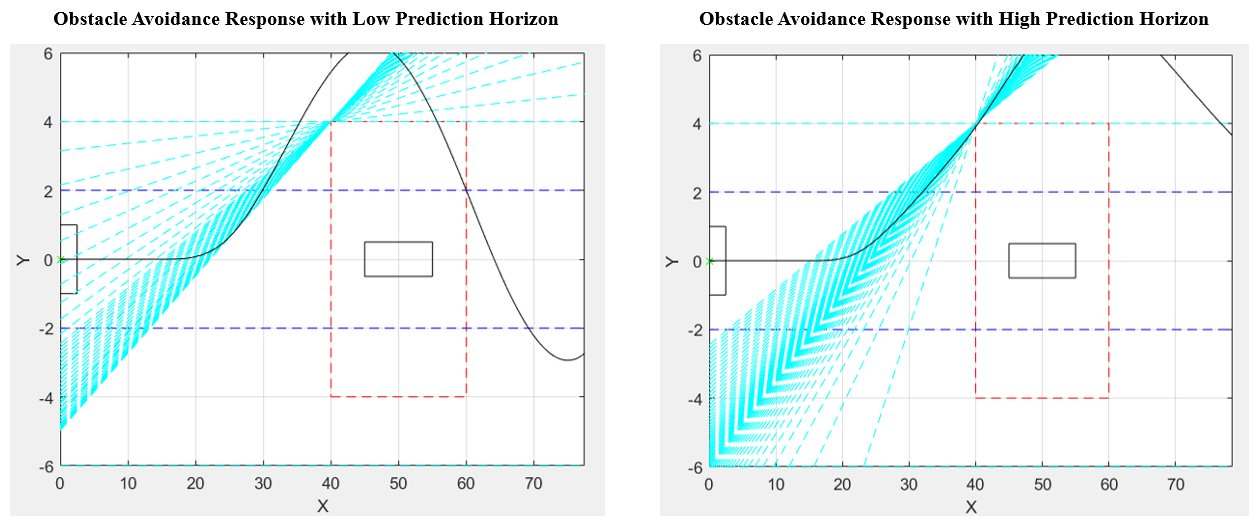
\includegraphics[width=\textwidth]{Images/high_vs_low_prediction_horizon.png}
\caption{Obstacle Avoidance Response for Low and High Prediction Horizons}
\end{figure}

\section{Model predictive controller for trajectory tracking and obstacle avoidance}
\paragraph{}
This section discusses a model that performs the driving tasks of tracking a reference trajectory, similar to the model outlined in section 4.1.3, as well as avoids obstacles in its path, much like the model discussed in section 4.1.4. This model has been implemented in Python using the \texttt{ipopt} library for solving the optimization problem. The model comprises several files which perform the following functions:
\begin{enumerate}[label = (\roman*), itemsep=-0.3em]
    \item \texttt{main.py}: the main model file, which loads the map \& simulation environment, sets up and solves the MPC problem, and plots the vehicle's position at each time step
    \item \texttt{MPC.py}: defines a class to store the characteristics of the MPC controller, get data regarding time-varying parameters (waypoints and lateral position errors), and generate obstacle constraints
    \item \texttt{model.py}: defines a class for the simple bicycle model and defines functions for model setup and getting the current waypoint from the reference path
    \item \texttt{reference\_path.py}: (adapted from an online GitHub repository$^{\text{[8]}}$) defines the \texttt{ReferencePath} class accessed in \texttt{main.py} and \texttt{model.py}
    \item \texttt{simulator.py}: (adapted from an online GitHub repository$^{\text{[8]}}$) defines the \texttt{Simulator} class used in \texttt{main.py}
    \item \texttt{map.py}: (adapted from an online GitHub repository$^{\text{[8]}}$) defines the \texttt{Map} and \texttt{Obstacle} classes use in \texttt{main.py}
    \item \texttt{globals.py}: defines global variables (distance covered by the vehicle and the prediction horizon) referenced by multiple files in the simulation
\end{enumerate}

\paragraph{}
Figure 4.12 illustrates the output response of the model at a particular time step. With each time step, the vehicle position is updated on the plot. The obstacle constraints and optimal control outputs are predicted by the MPC algorithm and updated on plot as well. As expected, the model results in a response that tracks the reference trajectory with a high accuracy, except for certain parts where it is forced to go off-track due to the presence of obstacles.

\begin{figure}[H]\label{fig4.12}
\centering 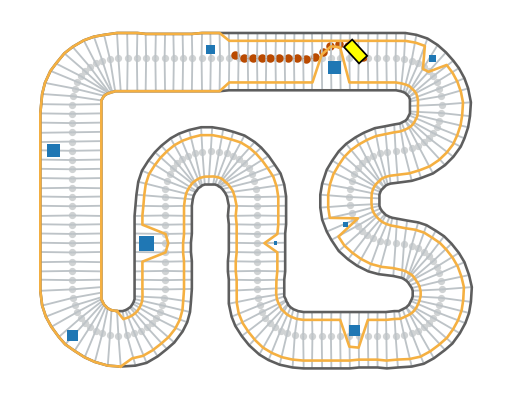
\includegraphics[scale=1]{Images/simulation_screenshot.png}
\caption{Trajectory Tracking and Obstacle Avoidance Response of MPC Controller (Python Simulation)}
\end{figure}
\chapter{Future Work}
\paragraph{}
The project work completed as part of Stage 1 of the project has resulted in significant insights into the impact of parameters such as vehicle velocity and the prediction \& control horizon on the behaviour of model predictive controllers. We have successfully implemented basic and adaptive controllers for two different driving tasks, namely trajectory tracking and obstacle avoidance. However, a significant amount of work remains to be done, which will be tackled in the next stage of the project. This includes, but is not limited to:
\begin{itemize}
    \item \textbf{Use of adaptive MPC for trajectory tracking around a racetrack}

    The model discussed in section 4.1.3 was locked to a specific pre-set value of vehicle velocity. This significantly hampered the response of the controller, since we were unable to adjust the vehicle's speed. A possible improvement to this model would be the inclusion of an adaptive MPC controller instead of a basic MPC controller, so that the vehicle states can be fed back to the controller to allow for adjustment of velocity as the vehicle turns along the track.
    \item \textbf{Employing non-linear MPC models}

    The continuous-time vehicle dynamics model is a non-linear one. Up till now, we have only looked at implementations of linear model predictive controllers, which required discretization to convert the non-linear model into a linear one that can be passed as an input to the controller. Though the output responses observed so far have been satisfactory, employing a non-linear MPC controller to be able to handle the continuous-time model without any need for discretization. This could potentially lead to performance improvements and better output responses.

    A major part of the future plan involves the exploration of non-linear MPC to incorporate a spatial bicycle model instead of the simple bicycle model we have been using so far. This will preclude the requirement of discretization, providing a more accurate tracking response. It will also allow for use of more complex tire models such as the Dugoff and Pacejka tire models for more precise computation of vehicle dynamics. 
    \item \textbf{Inclusion of image processing algorithms for obstacle detection}

    The obstacle avoidance algorithms discussed in sections 4.1.4 and 4.2 have relied on user-instantiated obstacles. While this is a convenient and less computationally expensive way of assessing the accuracy of a model, obstacles encountered by cars in the real world may not necessarily be pre-determined (e.g., landslides, construction work, etc). To account for this aspect of real-life obstacles, it is important to incorporate input from image sensors, such as cameras, LIDAR and SONAR sensors, in order to effectively locate any obstacles in the operational design domain of the ego vehicle. 
    
    With some additional processing, the sensor outputs can be converted into the obstacle's relative coordinates that can be used to generate obstacle constraints dynamically. The relevant models discussed section 4 can then be employed for the path planning task.

    \item \textbf{Inclusion of other actors in the self-driving environment}
    
    The simulations discussed in this report have included only the ego vehicle and obstacles, if any. We have not accounted for the presence of other actors in the self-driving environment, such as other vehicles and pedestrians. Hence, the models have been much less complex relative to an actual self-driving task. The inclusion of other actors in the surrounding environment would pose additional challenges for the optimal control problem. However, this would also provide a more accurate measure of how the controller would behave in the real world.

    This will be another major point of focus in the next stage of the project. 2-dimensional top-down simulations or 3-dimensional simulation will be carried out in open-source simulators, such as CARLA or Udacity's self-driving simulator, to demonstrate the effects of real-world driving aspects on MPC controller performance, including but not limited to traffic lights, pedestrian crossings and other vehicle actors in the operational design domain of the ego vehicle.

    \item \textbf{Implementation of reinforcement learning models for the path planning task}

    An alternative approach instead of employing a traditional feedback control system is the use of reinforcement learning algorithms for self-driving tasks. This would mean that the current system framework would be retired, in favour of a neural network that runs a reward-based optimization algorithm for controlling the vehicle. The training of such a type of self-driving algorithm is likely to take a significant amount of time, but it will reduce the number of post-training computations required. A reinforcement learning framework also means that the model learns from its earlier actions, which, in turn, would result in a generally superior ability to predict, follow and respond faster to previously encountered environmental changes as well as drastically reduce the number of repeated errors.
\end{itemize}

\noindent The possibilities mentioned above will be tackled as part of the project's next stage. Of course, this list is not exhaustive, and there may be other methods/improvements that may be discovered over the course of the project.
\chapter{References}
\section{Research Papers}
\begin{enumerate}
    \item Paolo Falcone, Francesco Borrelli, Jahan Asgari, Hongtei Eric Tseng. Predictive Active Steering Control for Autonomous Vehicle Systems. \textit{IEEE Transactions on Control Systems Technology}, 15(3), 2007.

    Link: \href{https://ieeexplore.ieee.org/document/4162483}{https://ieeexplore.ieee.org/document/4162483}
    \item Daisuke Akasaka, Taku Takahama. Model Predictive Control Approach to Design Practical Adaptive Cruise Control for Traffic Jam. \textit{International Journal of Automotive Engineering}, 9(3), 2018. 

    Link: \href{https://www.jstage.jst.go.jp/article/jsaeijae/9/3/9_20184095/_article}{https://www.jstage.jst.go.jp/article/jsaeijae/9/3/9\_20184095/\_article}
    \item Trieu Minh Vu, Reza Moezzi, Jindrich Cyrus, Jaroslav Hlava. Model Predictive Control for Autonomous Driving Vehicles. \textit{Electronics, MDPI Open Access Journals}, 10, 2021. 

    Link: \href{https://doi.org/10.3390/electronics10212593}{https://doi.org/10.3390/electronics10212593}
\end{enumerate}

\section{Other Resources}
\begin{enumerate}
    \setcounter{enumi}{3}
    \item Melda Ulusoy (2023). Designing an MPC controller with Simulink, MATLAB Central File Exchange. Retrieved October 11, 2023.

    Link: \href{https://www.mathworks.com/matlabcentral/fileexchange/68992-designing-an-mpc-controller-with-simulink}{https://www.mathworks.com/matlabcentral/fileexchange/68992}

    \item Melda Ulusoy (2023). Adaptive MPC Design with Simulink, MATLAB Central File Exchange. Retrieved October 11, 2023.

    Link: \href{https://www.mathworks.com/matlabcentral/fileexchange/68939-adaptive-mpc-design-with-simulink}{https://www.mathworks.com/matlabcentral/fileexchange/68939}
    \item Vehicle Path Tracking using Model Predictive Control (Improving Your Racecar Development), Mathworks GitHub Repository, 2022.

    Link: \href{https://in.mathworks.com/videos/vehicle-path-tracking-using-model-predictive-control-1647494222398.html}{https://in.mathworks.com/videos/vehicle-path-tracking-using-model-predictive-control}
    \newpage
    \item Obstacle Avoidance Using Adaptive Model Predictive Control, Mathworks Help Center (Automated Driving Applications, Model Predictive Control).

    Link: \href{https://in.mathworks.com/help/mpc/ug/obstacle-avoidance-using-adaptive-model-predictive-control.html}{https://in.mathworks.com/help/mpc/ug/obstacle-avoidance-using-adaptive-model-predictive-control}
    \item Multi-Purpose-MPC, Online GitHub Repository owned by \href{https://github.com/matssteinweg}{\texttt{matssteinweg}}, 2019.

    Link:
    \href{https://github.com/matssteinweg/Multi-Purpose-MPC}{https://github.com/matssteinweg/Multi-Purpose-MPC}
    \item Automated Driving using Model Predictive Control, Mathworks Help Center (Model Predictive Control Toolbox, Automated Driving Applications)

    Link: \href{https://in.mathworks.com/help/mpc/ug/automated-driving-using-model-predictive-control.html}{https://in.mathworks.com/help/mpc/ug/automated-driving-using-model-predictive-control}
    \item Jarrod M. Snider, Automatic Steering Methods for Autonomous Automobile Path Tracking, \textit{Robotics Institute, Carnegie Mellon University}, 2009.

    Link: \href{https://www.ri.cmu.edu/pub_files/2009/2/Automatic_Steering_Methods_for_Autonomous_Automobile_Path_Tracking.pdf}{https://www.ri.cmu.edu/pub\_files/2009/2/Automatic\_Steering\_Methods\_for\_Autonomous\_Automobile\newline\_Path\_Tracking.pdf}
    \item 
\end{enumerate}
%\backmatter
% \cleardoublepage
% \appendix

% \addcontentsline{toc}{chapter}{Appendix A}
% \chapter*{Appendix A}

% \cleardoublepage

% \addcontentsline{toc}{chapter}{Appendix B}
% \chapter*{Appendix B}


\end{document}